\clearpage

\lehead[]{\normalfont\sffamily\hspace*{-2.00cm}\textcolor{white}{\colorbox{lightblue}{\parbox[c][0.70cm][b]{1.60cm}{
\makebox[1.60cm][r]{\thechapter}\\ \makebox[1.60cm][r]{ÜBUNG}}}}\hspace{0.17cm}\textcolor{lightblue}{\chaptertitle}}
\rohead[]{\textcolor{lightblue}{\chaptertitle}\normalfont\sffamily\hspace*{0.17cm}\textcolor{white}{\colorbox{lightblue}{\parbox[c][0.70cm][b]{1.60cm}{\thechapter\\
ÜBUNG}}}\hspace{-2.00cm}}
%\chead[]{}
\rehead[]{\textcolor{lightblue}{AvHG, Inf, My}}
\lohead[]{\textcolor{lightblue}{AvHG, Inf, My}}

\section{Strings -- Übungen}

\subsection{Aufgabe 1: Vergleich von Strings}

\begin{compactenum}[a)]
\item Was wird in dem folgenden Code ausgegeben?

\begin{lstlisting}
public void paintComponent(Graphics g) {
    String s1 = "Hallo";
    String s2 = "Hallo";
    String s3 = "Hal";
    s3 += "lo";
    if (s1 == s2) {
        g.drawString("s1 und s2 sind gleich", 20,100);
    } else {
        g.drawString("s1 und s2 sind nicht gleich", 20,100);
    }
    if (s1 == s3) {
        g.drawString ("s1 und s3 sind gleich", 20,150);
    } else {
        g.drawString ("s1 und s3 sind nicht gleich", 20,150);
    }
}
\end{lstlisting}

\item Wie muss der Code abgeändert werden, damit ein echter Vergleich der
Zeichenketten durchgeführt wird?
\end{compactenum}


\subsection{Aufgabe 2: String-Operationen}

Wie ändert sich die Zeichenkette \lstinline|result| in dem folgenden Code?
Welcher Text wird am Ende ausgegeben?

\begin{lstlisting}
public void paintComponent (Graphics g) {
    String original = "software";
    String result;

    result = " hallo ";                               æ// Schritt 1
æ    result = result.replace('l',original.charAt(6));  æ// Schritt 2
æ    result = result.trim();                           æ// Schritt 3
æ    int index = original.indexOf('t');
    result = result.substring(0,index);               æ// Schritt 4
æ    result += "d";                                    æ// Schritt 5
æ    result = result.toUpperCase();                    æ// Schritt 6
æ    result += original.substring(4);                  æ// Schritt 7
æ
    g.drawString(result, 20, 30);
}
\end{lstlisting}


\subsection{Aufgabe 3: Noch mehr String-Operationen}

Füge in die nachfolgenden Code-Auszüge jeweils geeignete Aufrufe von
\myClass{String}-Methoden ein.

\begin{compactenum}[a)]
\item
\begin{lstlisting}
String s1 = "hallo";
String s2 = "  HALLO ";

æ/* Abschneiden der Leerzeichen von String s2 */



/* Vergleich der Strings ohne Berücksichtigung von Groß- und    
   Kleinschreibung */
æ
if (								) {
    System.out.println("Die Strings sind gleich");
}
\end{lstlisting}

\item Wandle die beiden Zahlen in Strings um und hänge beide Strings zu
einem Text aneinander (Ergebnis soll ein String mit dem Inhalt "1122"\ sein). 
\begin{lstlisting}
int zahl1 = 11;
int zahl2 = 22;
\end{lstlisting}
\end{compactenum}


\subsection{Aufgabe 4: Initialen}

Schreibe ein Programm, das die Initialen eines Namens ermittelt. 

Der \myClass{JFrame} enthält ein Textfeld zur Eingabe des Namens, einen Button,
mit dem die Berechnung gestartet wird, und ein nicht-editierbares Textfeld zur
Ausgabe der Initialen.

Der Benutzer gibt in dem ersten Textfeld einen Namen ein. Zum Beispiel:

Emil Anton Müller-Bruckner

Wenn er auf den Button drückt, schreibt das Programm in das zweite Textfeld die
Initialen des Namens. In diesem Beispiel:

EAMB


\subsection{Aufgabe 5: Rechnen mit versteckten Zahlen}

Im \myClass{JFrame} gibt es zwei Textfelder, in die der Benutzer Zahlen eingeben
soll.

Wenn der Benutzer auf einen Button drückt, werden die Zahlen addiert.

In einem \myClass{JTextField} kann der Benutzer natürlich auch falsche Werte
eintragen. Zum Beispiel könnte er versehentlich in eines der Textfelder
Buchstaben eingeben. Wenn man einen Text, der Buchstaben enthält, mit der
Methode \lstinline|parseInt()| der Klasse \myClass{Integer} in eine Zahl
konvertieren will, erzeugt das Programm einen Laufzeitfehler vom Typ
\myClass{NumberFormatException}.

Ein gutes Programm muss den Fehler also abfangen. Schreibe ein Programm, das
alle Buchstaben und Sonderzeichen aus den eingegebenen Zeichenketten entfernt
und nur die eingegebenen Ziffern auswertet. Wenn der Benutzer keine Ziffer in
ein \myClass{JTextField} eingegeben hat, soll mit der Zahl 0 gerechnet werden.

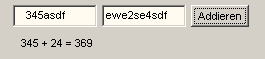
\includegraphics[width=0.4\textwidth]{./inf/SEKII/24_Java_GUI-Komponenten/RechnenMitVerstecktenZahlen.png}


\subsection{Aufgabe 6: Geheimbotschaft}

Es wurde vereinbart in einem ganz normalen Text eine geheime Botschaft zu
übermitteln. Die Geheimbotschaft erhält man, wenn man alle Buchstaben, die
hinter einem kleinen oder großen ’e’ stehen, aneinander fügt. Beispieltexte:

\begin{compactenum}[1.]
\item Tante Paula und Tante Anna sind erstaunlich nett. Gruß Meybritt.
\item Bitte fang im Februar ein Lama für mich!
\item Ehrlich sein ist schön. Meld dich bitte früh. Gruß Meerit.	
\item Emran und Anne Ohlmann sind mächtig. Erkundige dich mal.
\end{compactenum}

Tipp zur Entschlüsselung: Wandle zunächst alle Buchstaben des Textes in
Kleinbuchstaben um und lösche alle Zeichen aus dem Eingabe-String, die keine
Buchstaben sind.

\begin{center}
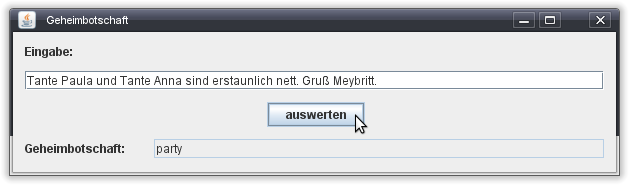
\includegraphics[width=0.85\textwidth]{./inf/SEKII/24_Java_GUI-Komponenten/Geheimbotschaft.png}
\end{center}